\documentclass[a4paper,12pt]{article}

\usepackage{tabularx} % Для автоподгона ширины
\usepackage{booktabs} % Для красивых линий \toprule, \midrule, \bottomrule
\usepackage[T2A]{fontenc}
\usepackage[utf8]{inputenc}
\usepackage[russian]{babel}
\usepackage{amsmath, amssymb}
\usepackage{graphicx}
\usepackage{geometry}
\usepackage{booktabs}
\geometry{left=30mm,right=15mm,top=20mm,bottom=20mm}
\usepackage{parskip}

\title{\textbf{Работа 2. Качественное определение белков}}\\


\begin{document}

\maketitle

\section*{Опыт 1. Разделение аминокислот методом хроматографии в тонком слое сорбента}

Метод базируется на различии в коэффициентах распределения аминокислот между подвижной органической фазой (н-бутанол -- уксусная кислота -- вода, $4:1:1$) и неподвижной водной фазой, связанной с сорбентом на пластинке «Силуфол».

\subsection*{Порядок выполнения:}
\begin{enumerate}
    \item На хроматографической пластинке «Силуфол» отмерить линию старта на расстоянии $1.5\text{ см}$ от нижнего края и линию фронта по факту остановки.
    \item Капиллярами нанести 2-3 капли анализируемой смеси и свидетелей аминокислот на линию старта.
    \item Поместить пластинку в хроматографическую камеру со смесью растворителей н-бутанол -- уксусная кислота -- вода ($4:1:1$).
    \item По достижении подвижной фазой линии фронта вынуть пластинку, прогреть на плитке для проявления пятен.
    \item Измерить расстояния, пройденные веществами ($L_{\text{вещ}}$) и растворителем ($L_{\text{фр}}$), и рассчитать значение $R_f$:
    \begin{equation}
    R_f = \frac{L_{\text{вещества}}}{L_{\text{фронта}}}
    \end{equation}
\end{enumerate}

По результатам ТСХ(фото в конце отчета) получилось определить, что в MIX содержится Tyr и какие-то еще другие (скорее всего две) аминокислоты. Пятно от Gly в MIX отсутствует, также были расчитаны значения $R_f$ для этих АК и неизвестных двух других АК(MIX1 и MIX2):

\begin{equation}
R_{Gly} = 0.194 \qquad  R_{Tyr} = 0.617 \qquad R_{MIX_1} = 0.081 \qquad  R_{MIX_2} = 0.306
\end{equation}

\newpage 
\section*{Опыт 2. Качественные реакции на белки}

\subsection*{Опыт 2.1. Биуретовая реакция (реакция Пиотровского)}
Специфична для пептидных связей ($-\text{CO}-\text{NH}-$). В щелочной среде ионы $\text{Cu}^{2+}$ образуют комплексное соединение с пептидными группами белков с характерным красно-фиолетовым окрашиванием ($\lambda_{\max} \approx 545\text{ нм}$).

\paragraph{А. Получение биурета и биуретовая реакция на биурет:}
При нагревании мочевины происходит дезаминирование с образованием биурета:
\begin{equation}
2\,\text{H}_2\text{N}-\text{CO}-\text{NH}_2 \xrightarrow{\Delta} \text{H}_2\text{N}-\text{CO}-\text{NH}-\text{CO}-\text{NH}_2 + \text{NH}_3\uparrow
\end{equation}
К полученному расплаву после охлаждения добавляют 1 М $NaOH$ и 0.1 М $CuSO_4$ до появления розово-красного окрашивания.

\begin{figure}[h]
  \centering
  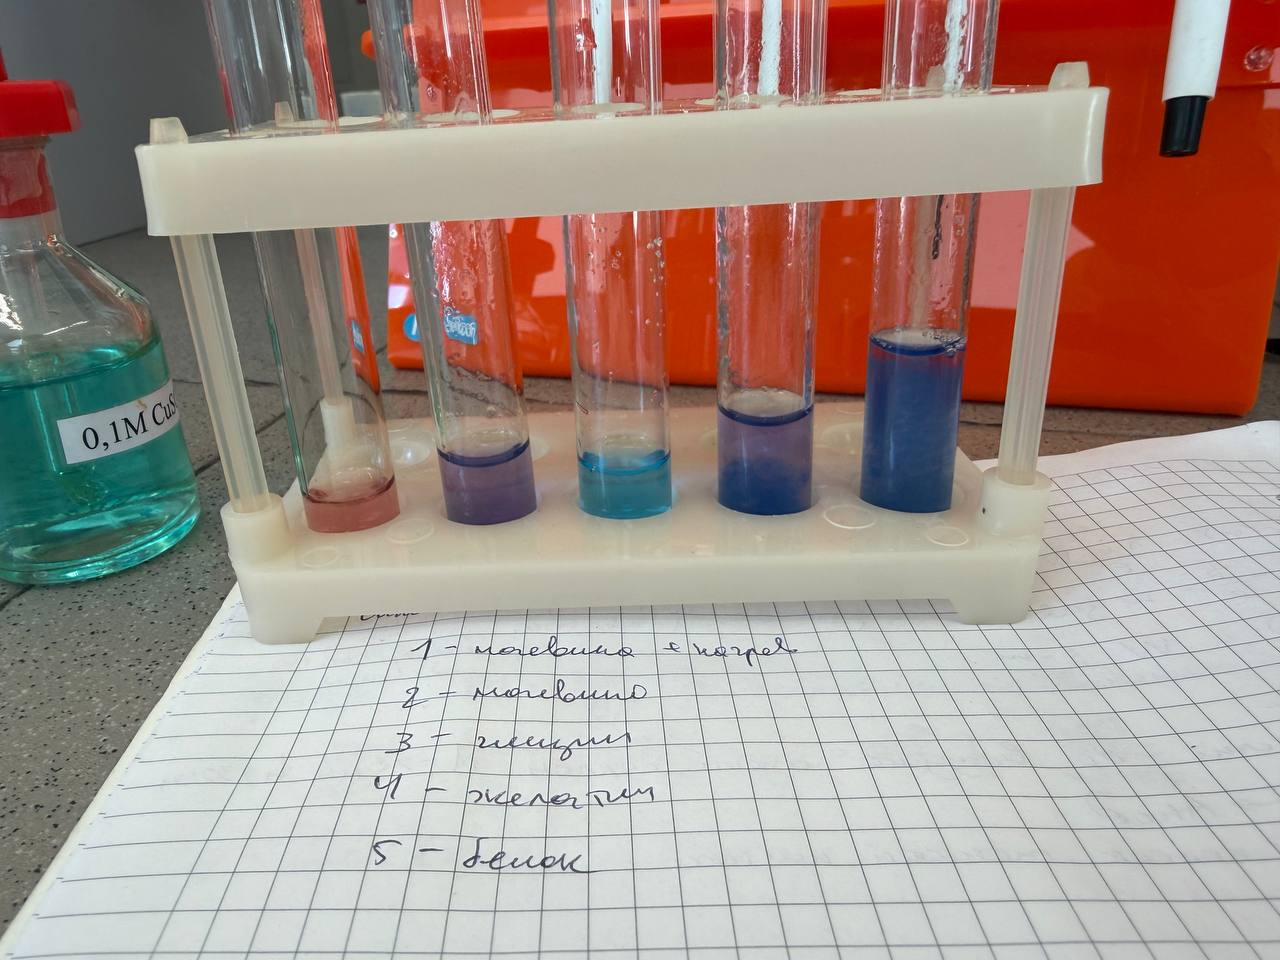
\includegraphics[width=0.8\textwidth]{Фотка1.jpg}
  \caption{Биуретовая реакция}
  \label{fig:myimage}
\end{figure}

\paragraph{Б. Биуретовая реакция на остальные растворы:}
К раствору мочевины, глицина, желатина и яичного белка добавляют $1\text{ мл}$ 1 М раствора $NaOH$ и $1\text{--}2$ капли 0.1 М раствора $CuSO_4$, полученные растворы приведены выше(рис.1). При этом все растворы дали характерную окраску (кроме глицина) образования соответствующих комплексов меди.

\newpage

\subsection*{Опыт 2.2. Нингидриновая реакция}
Универсальная реакция на свободные $\alpha$-аминогруппы. Интенсивность образующейся сине-фиолетовой окраски пропорциональна количеству свободных аминогрупп белка и может применяться в хроматографии для качественного и количественного анализа белков.

\begin{figure}[h]
  \centering
  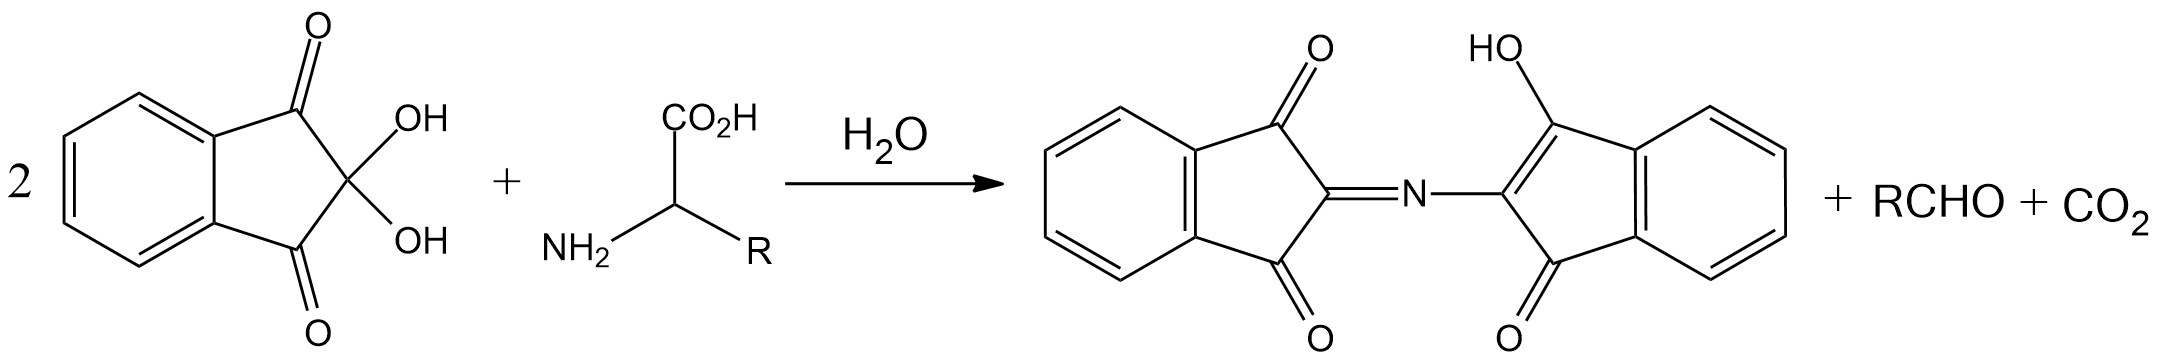
\includegraphics[width=1\textwidth]{нингидрин.png}
  \caption{Нингидриновая реакция}
  \label{fig:myimage}
\end{figure}

\paragraph{Порядок выполнения:}
К $1\text{ мл}$ раствора белка (или аминокислоты) добавляют $5\text{--}6$ капель $0.1\%$ водного раствора нингидрина и нагревают на кипящей водяной бане до появления сине-фиолетового окрашивания. Эксперименты были проведены с глицином, яичным белком и желатином: 1 - глицин, 2 - яичный белок, 3 - желатин (рис. 3).

\begin{figure}[h]
  \centering
  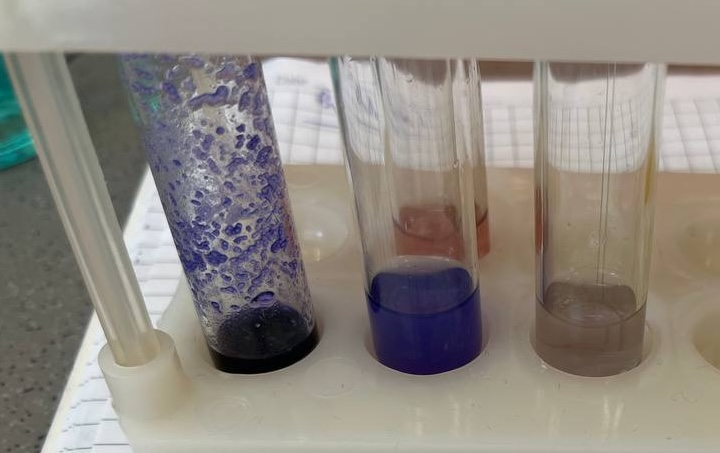
\includegraphics[width=0.8\textwidth]{нин_эксп.jpg}
  \caption{Нингидриновая реакция}
  \label{fig:myimage}
\end{figure}

Яркость окраски пропорциональна количеству свободных аминогрупп. Глицин содержит исключительно свободные АК и дает самую яркую окраску, яичный белок содержит сильно меньше свободных АК и поэтому окраска послабее. Желатин практически не дает окраску, так как желатин преимущественно состоит из пролина/оксипролина и глицина. Глицин образует пептидную цепь и поэтому не дает реакцию, а пролин вообще не образует пурпур Руэманна, так как содержит вторичный амин.

\newpage

\subsection*{Опыт 2.3. Ксантопротеиновая реакция}
Качественная реакция на ароматические аминокислоты (Tyr, Trp, Phe). Реакция заключается в введении одной или нескольких аминогрупп в ароматическое кольцо АК с образованием окрашенных нитропроизводных.

\begin{figure}[h]
  \centering
  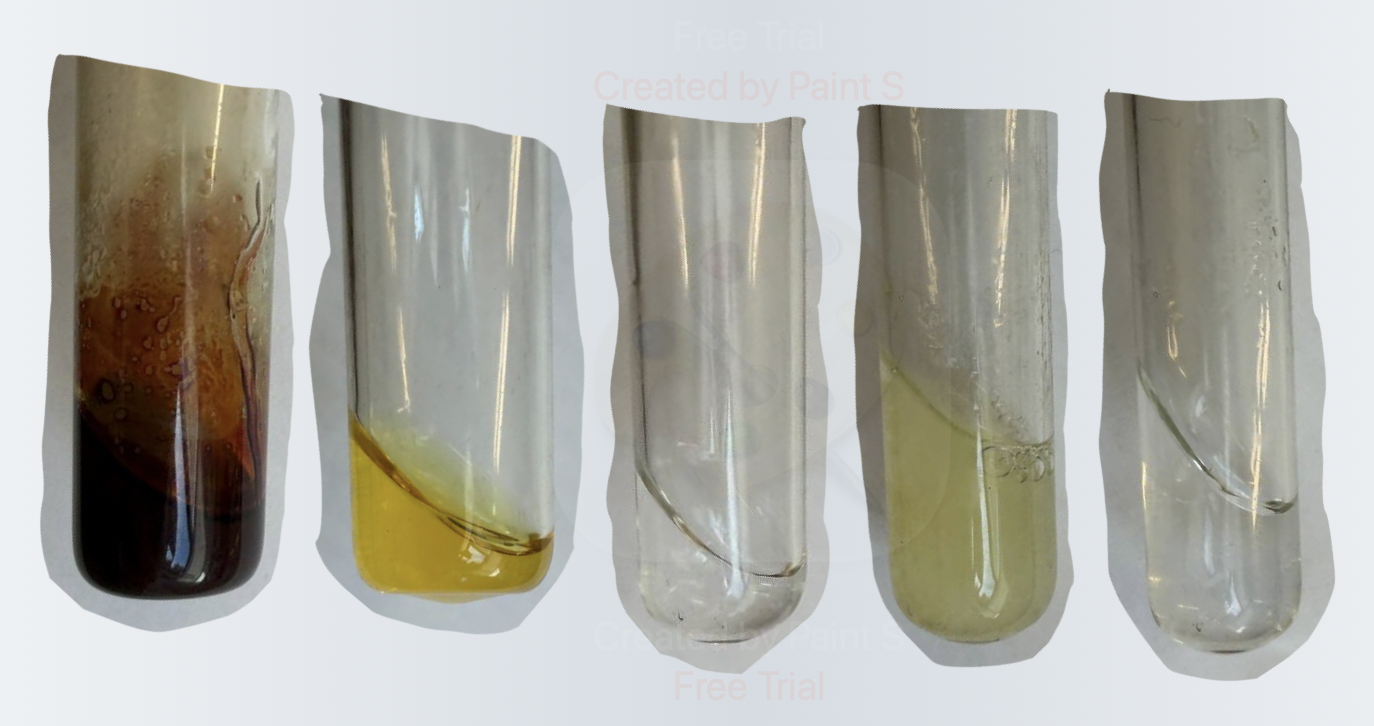
\includegraphics[width=0.8\textwidth]{ксан.png}
  \caption{Ксантопротеиновая реакция}
  \label{fig:myimage}
\end{figure}

\paragraph{Порядок выполнения:}
К $1\text{ мл}$ раствора белка/АК/фенола добавляют $5\text{--}6$ капель концентрированной $\text{HNO}_3$ и осторожно нагревают. Образуется осадoк/окрашивание желтого цвета. После охлаждения подщелачивают добавлением концентрированного аммиака или 1 М $NaOH$. 1 - фенол, 2 - тирозин, 3 - глицин, 4 - яичный белок, 5 - желатин (рис. 4). 

Фенол дает грязно-коричневую окраску за счет образования продуктов полинитрования фенола. У триптофана появляется желтакя окраска, которая и обусловлена образованием нитропроизводных АК. Глицин не содежрит ароматического кольца и не можеи давать реакции с азотной кислотой. Яичный белок немного пожелтел и денатурировал(за счет нагревания), это означает, что в яичном белке есть некоторое количество ароматических АК. Желатин не пожелтел, так как он состоит практически только из глицина и пролина. При добавлении к яичному белку раствора аммиака окраска практически не изменилась, скорее всего из-за низкой концентрации ароматических АК.


\newpage

\subsection*{Опыт 2.4. Реакция Фоля (на серосодержащие аминокислоты)}
Реакция Фоля позволяет определять белки/АК с содержанием Cys, Met и Cys-Cys, в ходе гидролиза образуются свободные сульфиды, которые дают коричневый осадок сульфида свинца при взаимодействии с его солями.
\begin{equation}
\text{NaH}\text{S} + \text{Pb}(\text{CH}_3\text{COO})_2 \longrightarrow \text{PbS}\downarrow (\text{черный/бурый}) + \,\text{CH}_3\text{COONa} + \text{CH}_3\text{COOH}
\end{equation}

\paragraph{Порядок выполнения:}
К $1\text{ мл}$ раствора белка добавляют $1\text{ мл}$ 1 М $NaOH$ и $1\text{--}2$ капли раствора ацетата свинца $\text{Pb}(\text{CH}_3\text{COO})_2$. Смесь кипятят $1\text{--}2$ минуты. 1 - яичный белок, 2 - желатин, 3 - яичный белок после центрифугирования (рис. 5).

\begin{figure}[h]
  \centering
  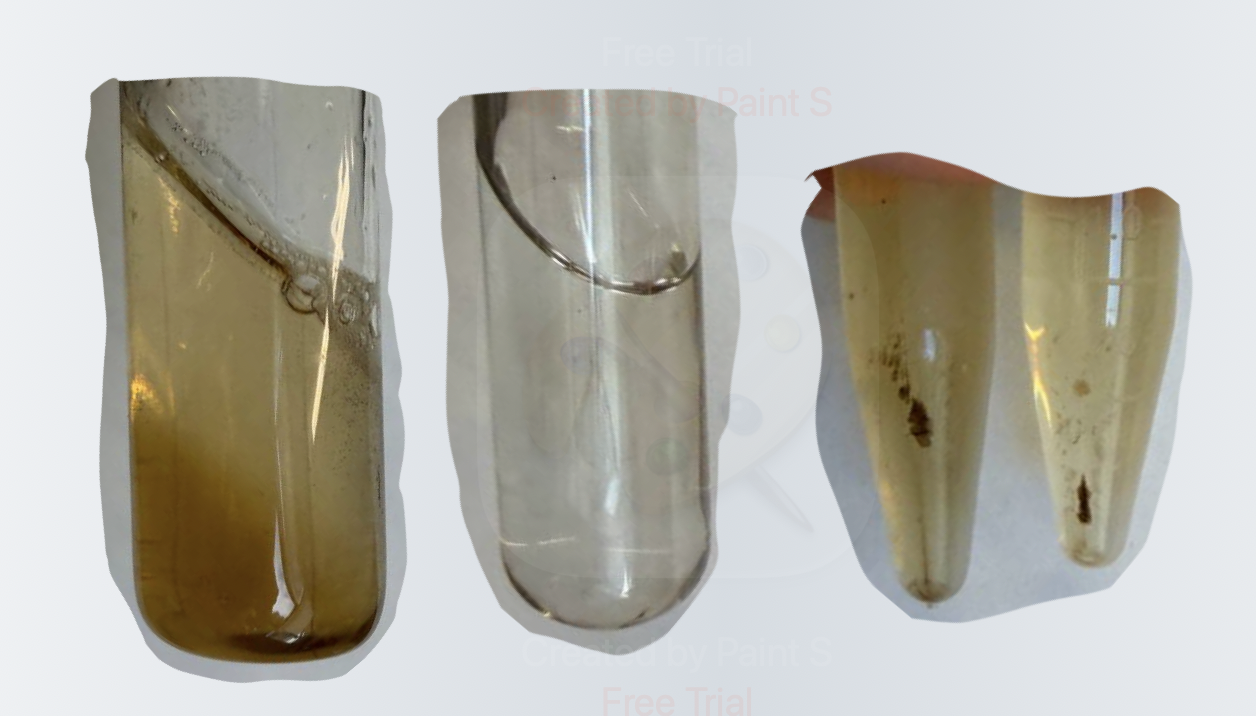
\includegraphics[width=0.6\textwidth]{фоль.png}
  \caption{Реакция Фоля}
  \label{fig:myimage}
\end{figure}

Как и говорилось ранее, в желатине практически отсутствуют серосодержащие АК и поэтому раствор прозрачный. В яичном белке соедржатся эти АК и поэтому дают коллоидный раствор из частиц сульфида свинца, для подтверждения того, что он действительно есть, мы провели центрифугирование.

\newpage

\section*{Опыт 3. Физико-химические свойства белков}

\subsection*{Опыт 3.1. Определение изоэлектрической точки белка}
Изоэлектрическая точка (pI) соответствует значению pH, при котором суммарный заряд белковой молекулы равен нулю, а растворимость минимальна.

\paragraph{Порядок выполнения:}
Готовят серию из 5 пробирок с ацетатным буфером различных pH. В каждую добавляют равное количество раствора желатина (1 мл), примерно 5 мл этилового спирта и после 5-10 минут, оценивают степень помутнения (рис. 6).

\begin{table}[h!]
\centering
\caption{Экспериментальные данные по определению pI желатина}
\vspace{2mm}
\resizebox{\textwidth}{!}{%
\begin{tabular}{ccccccc}
\toprule
№ пробирки & $V(\text{0.1M AcOH})$, мл & $C(\text{AcOH})$, М & $V(\text{0.1M AcONa})$, мл & $C(\text{AcONa})$, М & pH & Степень мутности \\
\midrule
1 & 1.8 & 0.09 & 0.2 & 0.01 & 3.81 & $+$ \\
2 & 1.6 & 0.08 & 0.4 & 0.02 & 4.16 & $++$ \\
3 & 1.0 & 0.05 & 1.0 & 0.05 & 4.76 & $+$ \\
4 & 0.4 & 0.02 & 1.6 & 0.08 & 5.36 & $-$ \\
5 & 0.2 & 0.01 & 1.8 & 0.01 & 5.71 & $-$ \\
\bottomrule
\end{tabular}%
}
\end{table}

\begin{figure}[h]
  \centering
  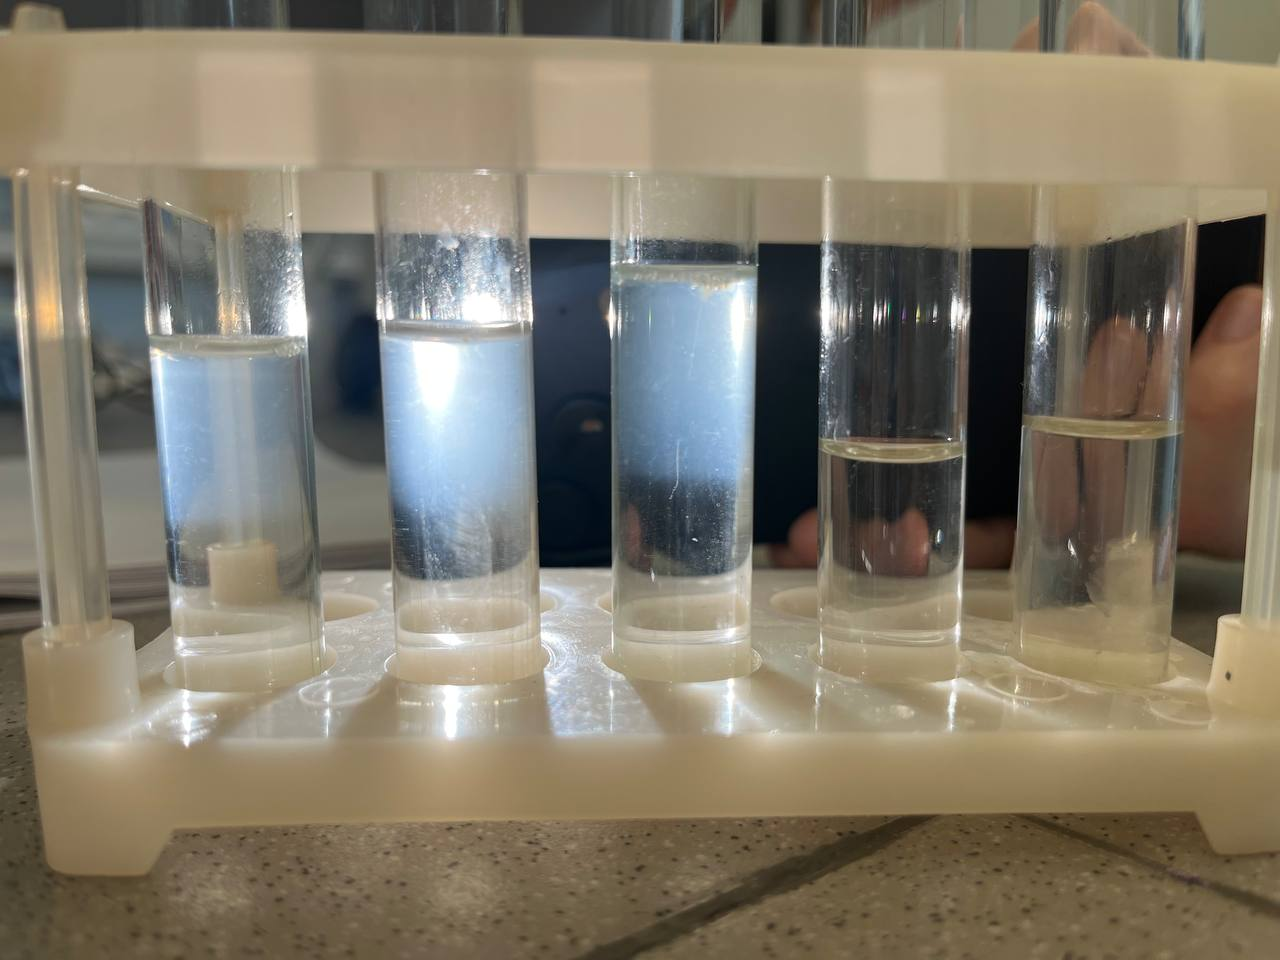
\includegraphics[width=0.6\textwidth]{мутность.jpg}
  \caption{Определение изоэлектрической точки}
  \label{fig:myimage}
\end{figure}

Получаем, что $pH = 4.16$ ближе всего к изоэлектрической точке желатина.

\newpage
\subsection*{Опыт 3.2. Высаливание белков}
Высаливание происходит при нейтрализации заряда белковой глобулы и под действием высокой ионной силы соли, снимающей гидратную оболочку. В щелочи ($NaOH$) белок переходит в растворимую форму из-за появления отрицательного заряда и электростатического отталкивания.

\textbf{Порядок выполнения:} К 1~мл раствора белка в первой пробирке прилили 1~мл насыщенного $(NH_4)_2SO_4$, во второй --- 1~мл $H_2O$. По каплям добавили 2M $HCl$. В смеси с солью выпал обильный осадок белка. Осадок разделили: при добавлении $H_2O$ он не растворился, при добавлении 1M $NaOH$ --- полностью растворился.

\vspace{0.3cm}

\subsection*{Опыт 3.3. Тепловая денатурация белков}

Нагревание вызывает денатурацию за счет разрыва нековалентных связей: глобула разворачивается, наружу выходят гидрофобные группы, формирующие нерастворимые агрегаты. Концентрированная щелочь (6M $NaOH$) депротонирует функциональные группы, сообщая высокий отрицательный заряд и разрушая агрегаты.

\textbf{Порядок выполнения:} 1~мл раствора белка нагрели на водяной бане до кипения (образовался плотный белый осадок) и охладили. Добавление 1~мл $H_2O$ не растворило осадок. Смесь разделили: при прибавлении 1~мл 6M $NaOH$ осадок полностью растворился.

\vspace{0.3cm}

\subsection*{Опыт 3.4. Осаждение белков органическими растворителями}

Органические растворители (ацетон) обладают низкой диэлектрической проницаемостью и высокой гидрофильностью. Они дегидратируют белок, связывая свободную воду, что в сочетании с подкислением до $pI$ вызывает мгновенную агрегацию и необратимую денатурацию.

\textbf{Порядок выполнения:} К 1~мл раствора белка прилили 1~мл насыщенного $(NH_4)_2SO_4$ и по каплям 2M $HCl$ до легкой мути. По стенке осторожно наслоили 1~мл ацетона. На границе фаз образовалось белое кольцо осадка, не растворяющееся при разбавлении водой.

\begin{figure}[h]
  \centering
  \begin{minipage}[c]{0.45\textwidth}
    \centering
    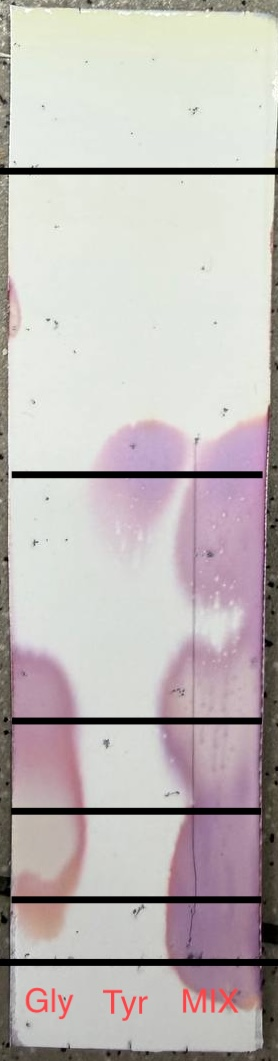
\includegraphics[width=0.5\textwidth]{ТСХ.jpg}
    \caption{Анализ ТСХ}
  \end{minipage}
  \hfill
  \begin{minipage}[c]{0.45\textwidth}
    \centering
    
\includegraphics[width=0.5\textwidth]{ТСХ_2.png}
    \caption{Пластинка ТСХ}
  \end{minipage}
\end{figure}

\end{document}